\documentclass[xcolor=dvipsnames]{beamer}

\mode<presentation>
{
  \usetheme{Frankfurt}
  % or ...

  \setbeamercovered{transparent}
  % or whatever (possibly just delete it)

  %\usecolortheme[named=Brown]{structure}

}

\usepackage[english]{babel}
\usepackage[utf8x]{inputenc}
%\usepackage[latin1]{inputenc}
\usepackage{times}
\usepackage[T1]{fontenc}
\usepackage{array,booktabs,tabularx}
\newcolumntype{Z}{>{\centering\arraybackslash}X} % centered tabularx columns
\newcommand{\pphantom}{\textcolor{ta3aluminium}} % phantom introduces a vertical space in p formatted table columns??!!
\usepackage{amsmath,amsthm, amssymb, latexsym}
\usepackage{graphicx}
\usepackage{verbatim}

\title[] {Implementación HW/SW de Arquitecturas de Clasificación de Paquetes Sobre Lógica Reconfigurable.}

\author[] {Jairo N. Trad y Luis R. Romano}


\institute[Universidades] % (optional, but mostly needed)
{
  \scriptsize Laboratorio de Comunicaciones Digitales \\
  \scriptsize Universidad Nacional de Córdoba, Facultad Ciencias Exactas, Físicas y Naturales \\ 
}

\AtBeginSubsection[]
{
  \begin{frame}<beamer>{Agenda}
  %  \scriptsize
    \tiny	
    \tableofcontents[currentsection,currentsubsection]
  \end{frame}
}

% If you wish to uncover everything in a step-wise fashion, uncomment
% the following command: 

%\beamerdefaultoverlayspecification{<+->}

\begin{document}

\begin{frame}
  \titlepage
\end{frame}

\begin{frame}{Agenda}
  \tiny	
  \tableofcontents
  % You might wish to add the option [pausesections]
\end{frame}

\scriptsize

\section{Motivación}

\subsection{Requerimientos}

\begin{frame}{Requerimientos de procesamiento en Redes}
  \scriptsize
  
  \begin{block}<+->{Características de Tráfico}

    \begin{itemize}
      \item Las redes de datos crecen en {\bf Complejidad:} nuevas aplicaciones, multimedia

      \item Las redes de datos crecen en {\bf Velocidad:} $n \times 100 Gbps\ (1Tbps@2015)$

      \item {\bf Consolidación} de múltiples servicios sobre redes Ethernet
      
      \item Redes \emph{Locales}, \emph{Metropolitanas} y \emph{Extensas} utilizan {\bf Conmutación de Paquetes}

      \item Adopción de tecnologías para \emph{virtualización} en redes y servidores
    \end{itemize}
    
  \end{block}
    
  \begin{block}<+->{Procesamiento de Paquetes}
    \begin{itemize}

      \item Los \emph{enlaces} ofrecen alta capacidad. El \emph{procesamiento} de paquetes es {\bf crítico} y debe optimizarse

      \item El procesamiento \emph{a velocidad de línea}

      \item Paquete Ethernet mínimo $=64 bytes$ $\rightarrow 6 nanosegundos/paquete$  
    \end{itemize}    
  \end{block}

\end{frame}



\subsection{Soluciones}
\begin{frame}{Soluciones}
  \begin{block}<+->{Granularidad}  
    \begin{itemize}
      \scriptsize
      \item {\bf Actualmente} $\rightarrow$ {\bf paquetes} de longitud {\bf variable}
      \item Peor caso $\rightarrow$ mínima longitud (64 bytes en Ethernet)
      \item {\bf Tendencia} $\rightarrow$ agregación de paquetes en {\bf flujos}
      \item Ejemplos: Multi-protocol Label Switching (MPLS), VLANs (802.1Q)  
    \end{itemize}
  \end{block}
    
  \vskip2ex  
%    \newcolumntype{V}{>{\centering\arraybackslash} m{.4\linewidth} }
    \begin{tabularx}{\linewidth}{ZZ}
    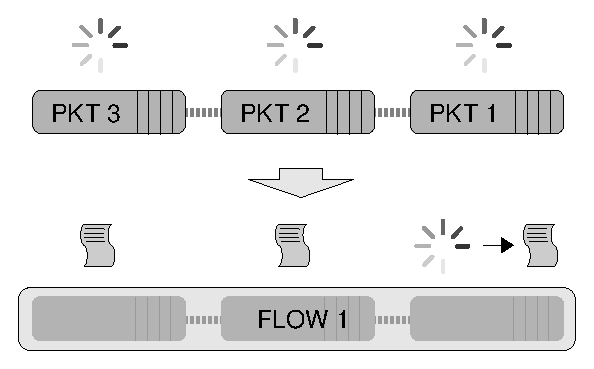
\includegraphics[scale=0.45]{figures/packet_vs_flow-crop.eps} 
    &
    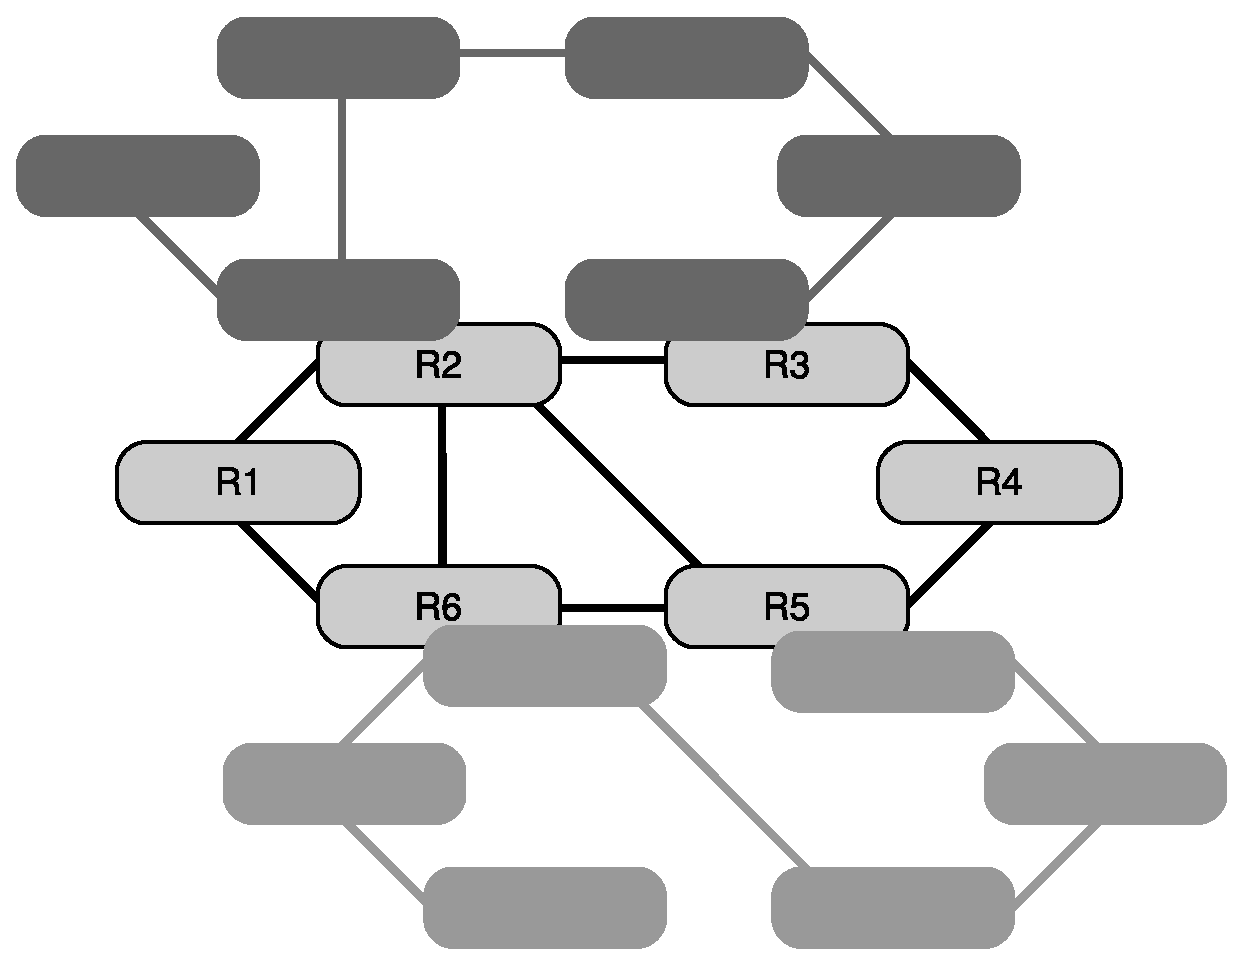
\includegraphics[scale=0.2]{figures/network_virtualization_2.eps}
    \\
    \tiny Agregacion de flujos
    &
    \tiny Virtualizacion de redes
    \\
  \end{tabularx}


\end{frame}  
  
   
\begin {frame}{Tecnologías Actuales}   
  
  Requerimientos $\rightarrow$ {\bf flexibilidad, performance} 
  
  \begin{block}<+->{Circuitos de Propósito Específico (ASICs)} 
    \begin{itemize}
      \scriptsize
      \item Cientos de bloques especializados trabajando en paralelo
      \item Alto desempeño. No programables, alto costo y tiempo de desarrollo.
    \end{itemize}
  \end{block}

  \begin{block}<+->{Procesadores de Red (NPs)}   
    \begin{itemize}
      \scriptsize
      \item Múltiples elementos de procesamiento, buena performance para ciertas tareas. IXP(Intel), PowerNP (IBM)
      \item Difícil portabilidad, interfaces propietarias
    \end{itemize}
  \end{block}

  \begin{block}<+->{Procesadores de Propósito General (GPPs)} 
    \begin{itemize}
      \scriptsize
      \item Arquitectura PC + Software especializado: \emph{Click}, \emph{Zebra/Xorp/Quagga}
      \item Alta flexibilidad, bajo costo. Limitación por transacciones con RAM y naturaleza secuencial
    \end{itemize}
  \end{block}
  
\end{frame}


\begin{frame}{Nuevas tecnologías}

  \begin{block}<+->{Dispositivos Lógicos Programables (FPGAs)} 
    \begin{itemize}
      \scriptsize
      \item Permiten \emph{reconfiguración} y \emph{reprogramación}, contando con librerías de \emph{Open Hardware}. 
      \item Su performance no es lejana a la de un ASIC. Fabricantes: Altera, Xilinx, Actel.
      \item Incorporación creciente de bloques \emph{hardcore} especializados
    \end{itemize}      
  \end{block}
    \vskip3ex
    \center 
    \newcolumntype{V}{>{\centering\arraybackslash} m{.3\linewidth} }
    \begin{tabularx}{\linewidth}{VVV}

      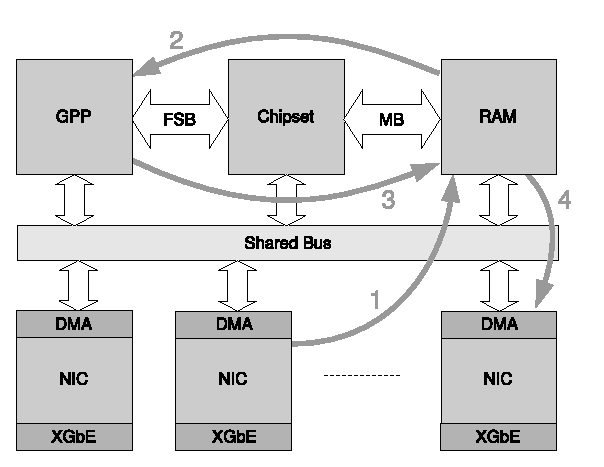
\includegraphics[scale=0.35]{figures/GPP_based.eps}
      &
      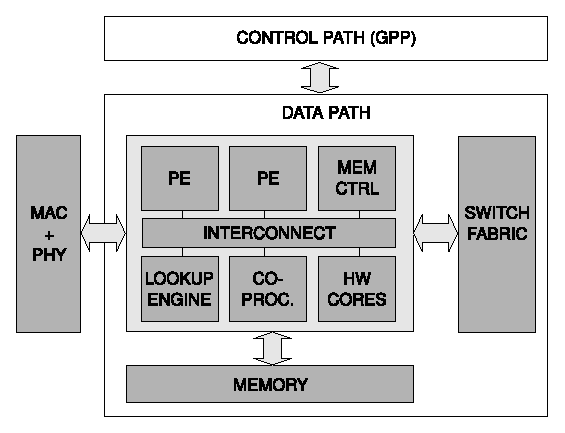
\includegraphics[scale=0.35]{figures/NP_based.eps}
      &
      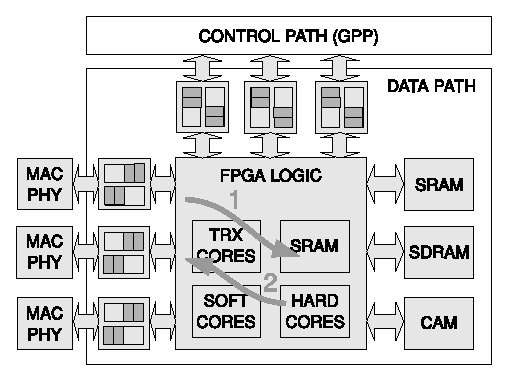
\includegraphics[scale=0.38]{figures/FPGA_based.eps}
      \\
      \tiny Implementación con GPPs
      &
      \tiny Implementación con NPs
      &
      \tiny Implementación con FPGAs
      \\
    \end{tabularx}
\end{frame}

\begin{frame}{FPGA como plataforma para SoC}

  \begin{block}<+->{Sistema en un Chip(SoC)} 
    \begin{itemize}
      \scriptsize
      \item Son circuitos integrados que contienen todo, o la mayoria, de los modulos que componen un sistema informatico o electronico en un solo componente.
	%\item Se diferencian de los microcontroladores en que cuentan con una mayor cantidad de memoria, en general externa, permitiendo ejecutar aplicaciones mas grandes y complejas. 
    \end{itemize}      
  \end{block}

  \begin{block}<+->{FPGA como plataforma para SoC} 
    \begin{itemize}
      \scriptsize
      \item En la ultima decada la integracion entre FPGAs de proposito general y CPUs tuvo una aceptacion amplia como plataforma de para el desarrollo de SoC.    
	\item La flexibilidad, el prototipado rapido, el aumento de la cantidad de logica reprogramable de proposito general y la creciente disponibilidad de IP cores fueron elementos determinantes que profundizaron esta tendencia.
	\center
        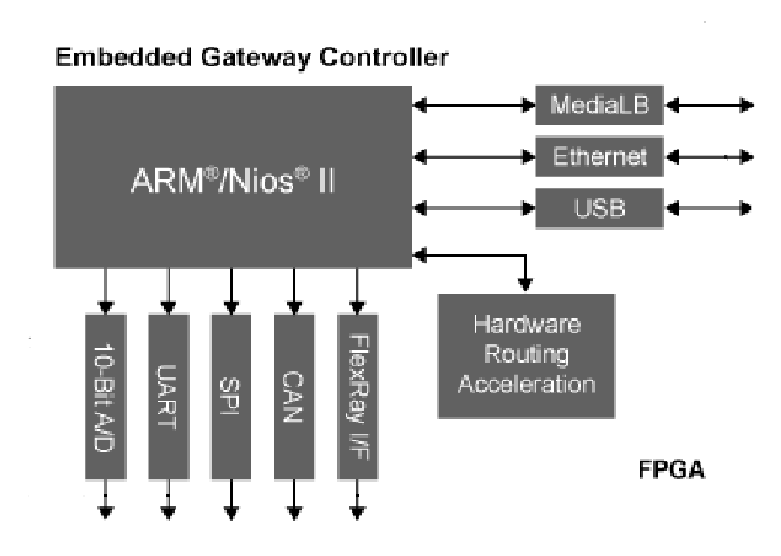
\includegraphics[scale=0.35]{figures/soc2.eps} 

    \end{itemize}      
  \end{block}
\end{frame}


\subsection{Problema marco}

\begin{frame}{Clasificación de Paquetes}

 \begin{block}<+->{Clasificación}   
    \begin{itemize}
      \scriptsize
      \item La necesidad de procesar cada vez más paquetes de datos lleva a lo que se conoce como \textit{clasificación.}
      \item Es el proceso de categorización de paquetes en distintos flujos.
      \item Efectuada en base a un número de campos de una cabecera.
      \item En general, para una clasificación basada en N campos, se dice que la misma es N-dimensional (o multidimensional) 
      \item Un caso en particular de la clasificación unidimensional (N=1) utilizando el campo IP destino es lo que se conoce como \textit{IP Lookup}.     
    \end{itemize}
  \end{block}
\end{frame}

\begin{frame}{Dirección IP - Prefijos}
 \begin{block}<+->{Dirección IP}   
    \begin{itemize}
      \scriptsize
      \item Es un número de 32 bit que identifica un dispositivo dentro de una red que utilice el protocolo IP
      \item Estructura jerárquica. Una parte de la dirección corresponde a la red, y la otra al host dentro de la red
      \item Los bits que corresponden a la parte de red conforman lo que se denomina \textit{prefijo de red}.
     \end{itemize}
  \end{block}
\begin{block}<+->{Formas de representar un prefijo de red}   
    \begin{itemize}
      \scriptsize
      \item Binario con asterisco (132.239 - 1000010011101111*)
      \item Notación A/L, donde A es una dirección IP y L es la longitud del prefijo (132.239.0.0/16)
      \item Notación máscara: se utiliza una dirección de red y una máscara (132.239.0.0 con máscara 255.255.0.0)
     \end{itemize}
  \end{block}
\end{frame}

\begin{frame}{IP LookUp}
 \begin{block}<+->{IP Lookup}   
    \begin{itemize}
      \scriptsize
      \item Se lleva a cabo en el dispositivo de enrutamiento.
      \item Un paquete llega por una interfaz de entrada. Éste porta una dirección IP de destino determinada.
      \item El dispositivo consulta una tabla para determinar la interfaz de salida para el paquete en cuestión
      \item Dicha tabla contiene un conjunto de prefijos con sus correspondientes interfaces de salida.
      \item El paquete es correspondido con el prefijo más largo que esté contenido en la dirección de destino y luego es redirigido  a la correspondiente interfaz de salida
      \item No es una busqueda trivial, ya que no se busca un valor en particular sino un prefijo contenido dentro de un valor. No aplican los algoritmos de búsqueda tradicionales.   
    \end{itemize}
  \end{block}
\end{frame}

\begin{frame}{Prefijos}
\center 
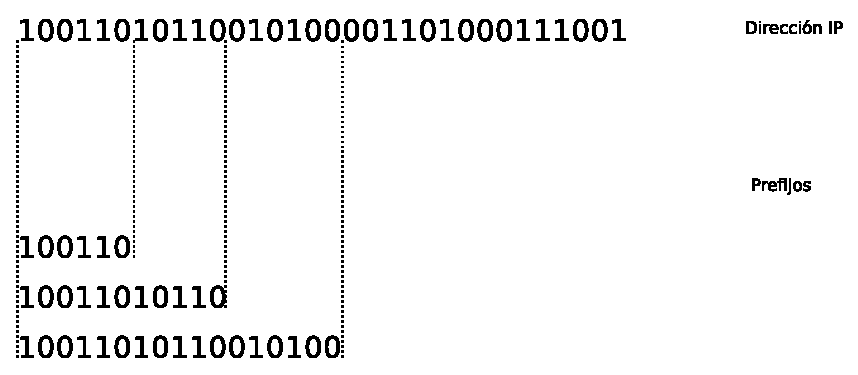
\includegraphics[scale=0.75]{figures/prefijos.eps}
\end{frame}

\subsection{Objetivos}
\begin{frame}{Objetivos}
\begin{block}<+->{Generales}   
    \begin{itemize}
      \scriptsize
      \item Estudiar los diversos algoritmos de clasificacion de paquetes para poder encontrar las limitaciones en la implementacion de los mismos.
      \item Considerar una plataforma de logica reprogramable que permita integrar arquitecturas de hardware con software embebido.
    \end{itemize}
  \end{block}
  
\begin{block}<+->{Específicos}   
    \begin{itemize}
      \scriptsize
     	\item Diseñar un sistema embebido que realice la clasificiación unidimensional de paquetes mediante una arquitectura mixta, Hardware-Software
	\item Implementar dicho sistema en hardware reconfigurable
	\item Implementar al menos 2 algoritmos conocidos y analizar su performance
	\item Sugerir mejoras en la implementación de los mismos   
    \end{itemize}
  \end{block}
\end{frame}

\section{Sistema}
\subsection{Solución Propuesta}
\begin{frame}{Solución}

    \begin{enumerate}
      \scriptsize
 \pause     	\item Un flujo de paquetes llega a la interfaz de red del dispositivo y es necesario clasificarlo en distintos flujos para que sea redireccionado.
\pause 	\item Se almacenan en un buffer los paquetes en orden de llegada.
\pause 	\item Se extrae el primer paquete y se toma la informacion que pertenece a la cabecera, la informacion completa del paquete queda en espera.
\pause 	\item Se envia al microprocesador la cabecera. 
\pause 	\item El Microprocesador aplica un algoritmo de clasificacion a cierta informacion de la cabecera y reenvia los resultados al Hardware. 
\pause 	\item Se anexa a cada palabra del paquete un Tag adjunto con el resultado de la clasificacion y se lo envia hacia la interfaz de salida.
    \end{enumerate}

\end{frame}

\begin{frame}{Arquitectura propuesta}
   \center 
   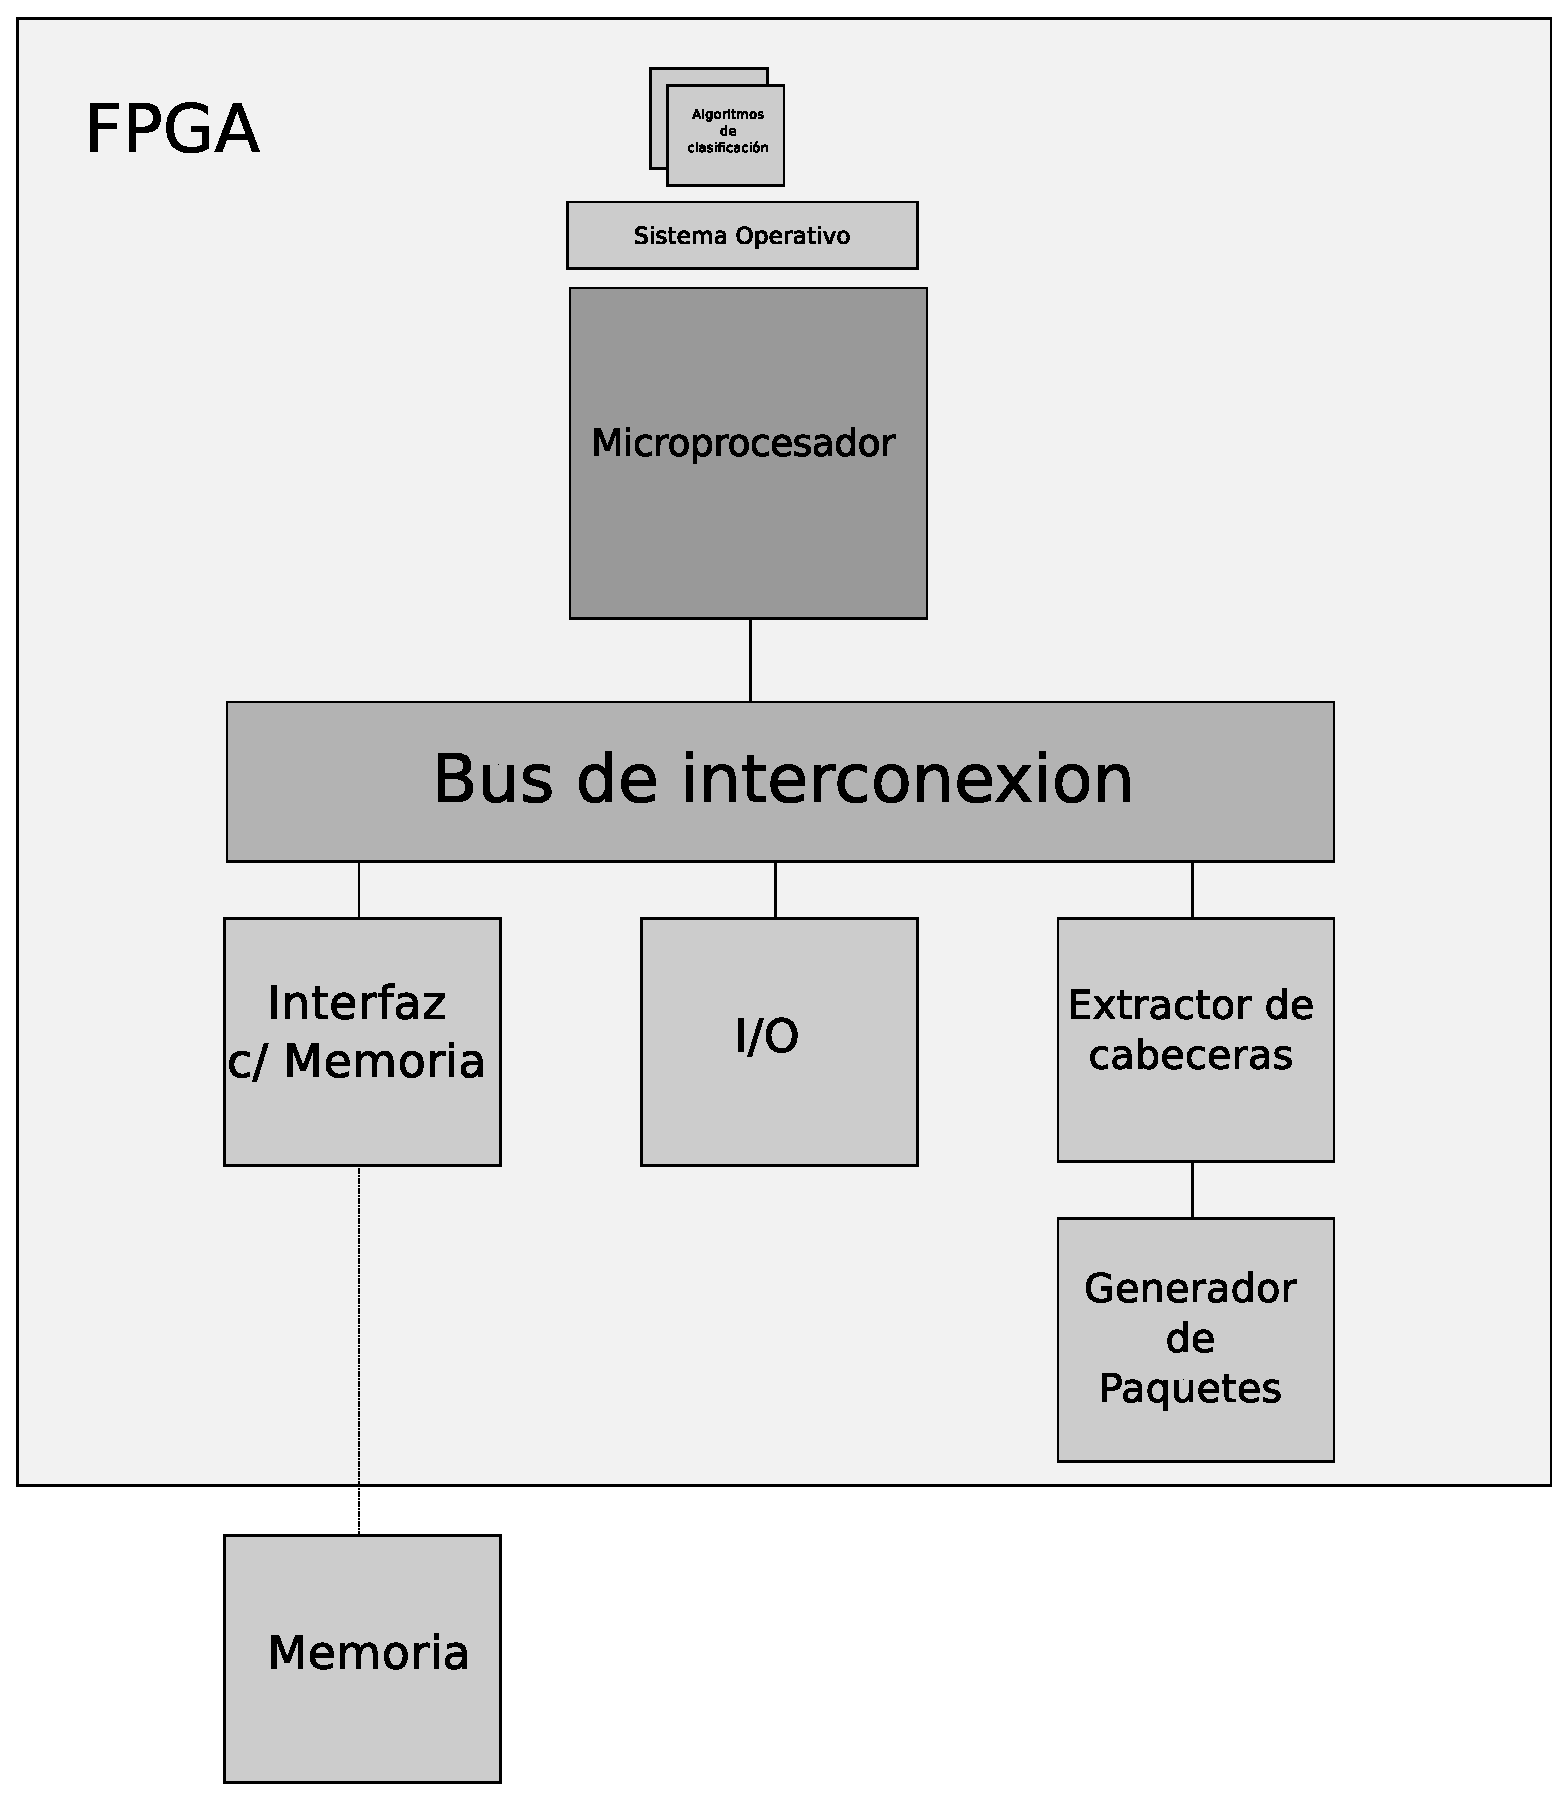
\includegraphics[scale=0.25]{figures/solucion.eps}
\end{frame}

\begin{comment}
\subsection{Descripcion funcional bloque a bloque}
\begin{frame}{Descripcion funcional}
\begin{block}<+->{Microprocesador}   
    \begin{itemize}
      \scriptsize
     	\item Recibe una cabecera y la procesa mediante la ejecución de un software de clasificación de paquetes.
    \end{itemize}
  \end{block}
  \begin{block}<+->{Bus de interconexión}   
    \begin{itemize}
      \scriptsize
     	\item Interconecta los componentes del sistema. 
    \end{itemize}
  \end{block}
\begin{block}<+->{Memoria}   
    \begin{itemize}
      \scriptsize
     	\item Almacena el software de clasificación de paquetes.
    \end{itemize}
  \end{block}
  \begin{block}<+->{Modulo extractor de cabeceras}   
    \begin{itemize}
      \scriptsize
     	\item Extrae una cabecera a partir de cada paquete recibido.
	\item La envía al software de clasificaciónd
	\item Recibe la información generada por dicho software
    \end{itemize}
  \end{block}
\end{frame}
\end{comment}

\subsection{Interfaz de Acceso a la Cabecera}

\begin{frame}{Interfaz de Acceso a la Cabecera}
\center 
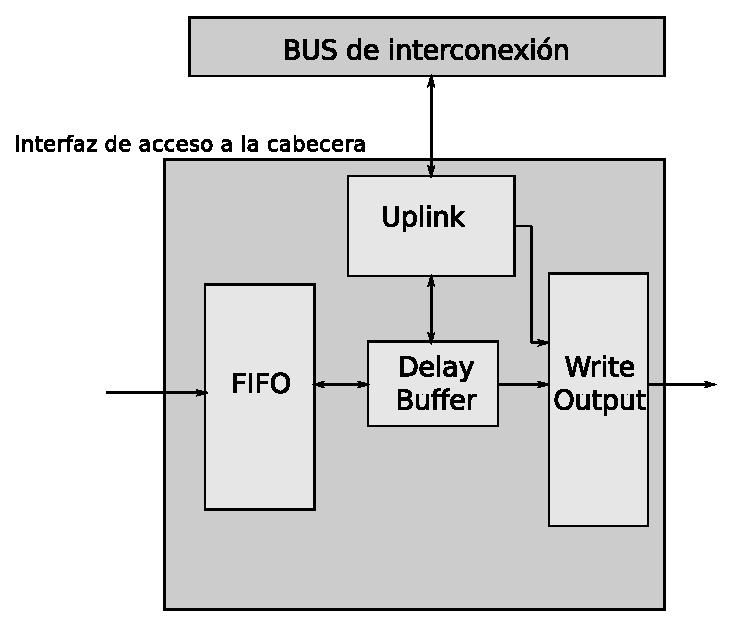
\includegraphics[scale=0.60]{figures/modulo.eps}
\end{frame}

\begin{frame}{Descripción funcional}

\begin{block}<+->{FIFO}   
    \begin{itemize}
      \scriptsize
     	\item Recibe los paquetes y los almacena en una memoria interna.
	\item De tamaño configurable.
    \end{itemize}
  \end{block}
\begin{block}<+->{Delay Buffer}   
    \begin{itemize}
      \scriptsize
     	\item Va tomando los datos desde la FIFO.
	\item Detecta inicio y finalización de cada paquete.
	\item Envía las primeras 5 palabras del paquete, suficientes para cubir la cabecera IP, a Uplink.
	\item Mantiene almacenado el paquete mientras el software toma una decisión.
    \end{itemize}
  \end{block}
\end{frame}
\begin{frame}{Descripción funcional (cont)}
  \begin{block}<+->{Uplink}   
    \begin{itemize}
      \scriptsize
     	\item Entiende las señales que maneja el Bus y puede interrumpir al Procesador.
	\item Genera interrupciones al procesador cuando los datos están disponibles.
	\item Puede enviar al procesador la cabecera completa o solo una parte, siempre en palabras de 32 bits.
	\item Cuando el procesador responde con el resultado de la clasificación, el mismo es almacenado y enviado al módulo Write Output
    \end{itemize}
  \end{block}
\begin{block}<+->{Write Output}   
    \begin{itemize}
      \scriptsize
     	\item Toma la salida de Delay Buffer.
	\item Escribe el resultado que le envía Uplink en la etiqueta que se encuentra anexa en cada una de las palabras del paquete.
    \end{itemize}
  \end{block}
\end{frame}

\subsection{Formato de la cabecera}
\begin{frame}{Formato de la cabecera}
 \center 
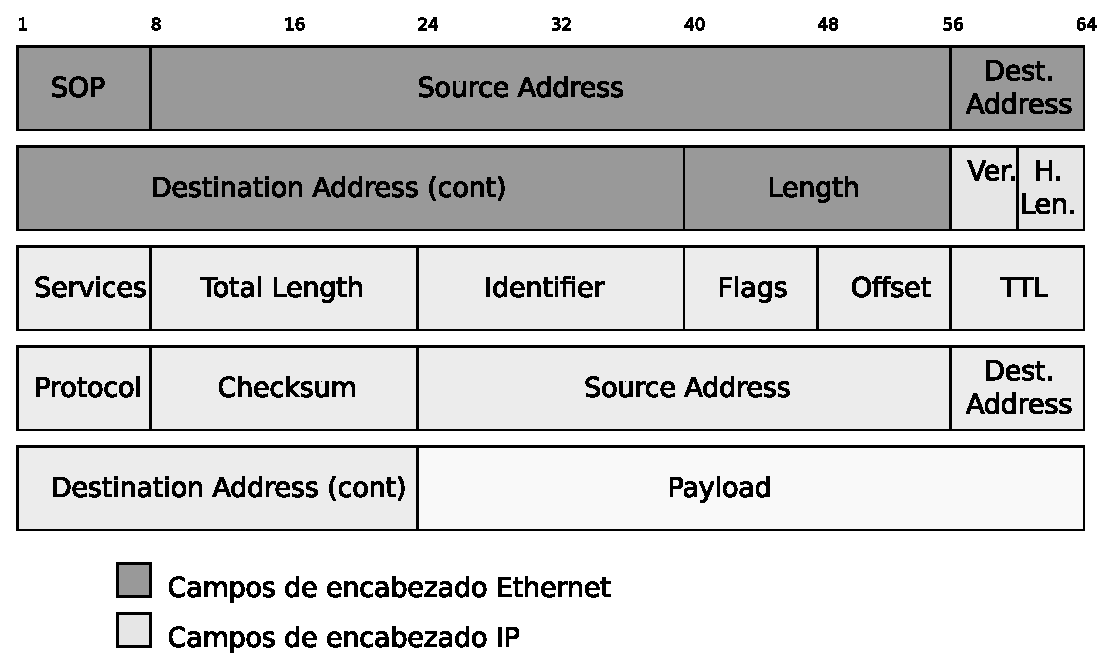
\includegraphics[scale=0.55]{figures/cabecera.eps}
\end{frame}

\subsection{Algoritmos de Clasificación}
\begin{frame}{Algoritmos de Clasificación}
\begin{block}<+->{Linear Lookup (LLU)}   
    \begin{itemize}
      \scriptsize
     	\item Prefijos almacenados en una lista enlazada
	\item Se toma como entrada una determinada dirección de destino y se va comparando nodo a nodo.
	\item Prefijos ordenados por longitud
	\item La primer coincidencia es la mejor
    \end{itemize}
  \end{block}
  \begin{block}<+->{Unibit trie lookup (UTL)}   
    \begin{itemize}
      \scriptsize
     	\item Prefijos almacenados en un arbol
	\item Cada nodo representa un bit del prefijo
	\item Se toma como entrada una dirección de destino y se va recorriendo el arbol en base a los bits
    \end{itemize}
  \end{block}
\end{frame}




\section{Arquitectura}
\begin{comment}
\subsection{Bus Avalon}
\begin{frame}{Bus Avalon}
  \begin{block}<+->{Avalon}   
    \begin{itemize}
      \scriptsize
     	\item Es una familia de interfaces provista por Altera
	\item Diferentes tipos, en base a las necesidades (ST, MM, Clock, Interrupt, Conduit, Reset)
    \end{itemize}
  \end{block}
\begin{block}<+->{En este diseño}   
    \begin{itemize}
      \scriptsize
     	\item Avalon MM $\rightarrow$ Los dispositivos están mapeados en memoria
	\item Avalon Clock Interface $\rightarrow$ Provee señal de clock al sistema
	\item Avalon Interrupt Interface $\rightarrow$ Permite que el módulo extractor de cabeceras interrumpa al procesador
	\item Avalon Conduit Interface $\rightarrow$ Permite visualizar resultados fuera de la FPGA
    \end{itemize}
  \end{block}
\end{frame}

\begin{frame}{Señales utilizadas}
  \begin{block}<+->{Avalon MM}
  \begin{itemize}
      \scriptsize
	\item address: Direcciona los datos enviados a o recibidos desde el procesador.
	\item chipselect: Se usa en combinacion con read o write.
	\item read: Indica una transferencia de lectura.
	\item readdata: Bus por el cual se transfieren los datos desde el preriférico hacia el procesador.
	\item write: Indica una transferencia de escritura.
	\item writedata: Bus por el cual se transfieren los datos desde el procesador hacia el periférico.
   \end{itemize}
\end{block}	

\begin{block}<+->{Avalon Clock Interface}
  \begin{itemize}
      \scriptsize
	\item clk: Provee clock para la sincronización de señales.	
   \end{itemize}
  \end{block}
\end{frame}

\begin{frame}{Señales utilizadas (cont)}
  \begin{block}<+->{Avalon Interrupt Interface}
  \begin{itemize}
      \scriptsize
	\item irq: Permite al modulo enviar una señal de interrupción al procesador cuando hay una cabecera lista para ser procesada.
   \end{itemize}
\end{block}	

\begin{block}<+->{Avalon Conduit Interface}
  \begin{itemize}
      \scriptsize
	\item export: Permite exportar señales "fuera" de la FPGA. En este caso, se la utiliza para visualizar ciertos resultados de la clasificación por medio del panel de LEDs de la placa de desarrollo.	
   \end{itemize}
  \end{block}
\end{frame}
\end{comment}

\subsection{Diagrama en bloques: Lineas E/S}
\begin{frame}{Generador}
\center 
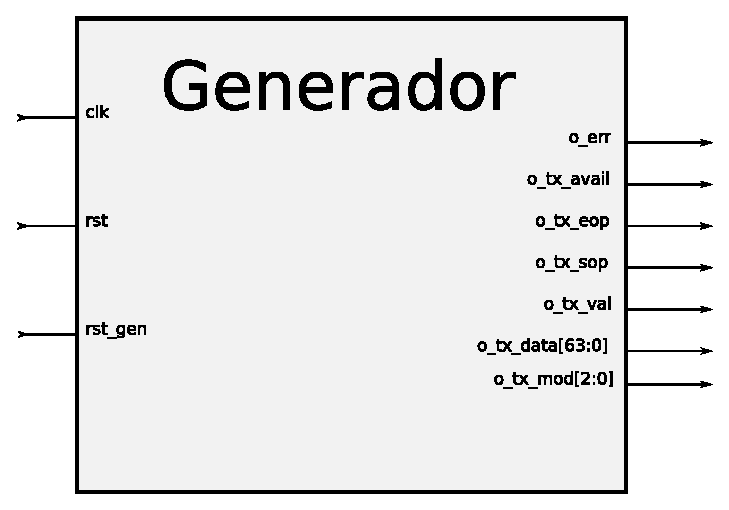
\includegraphics[scale=0.60]{figures/bloqgenerador.eps}
\end{frame}

\begin{frame}{FIFO}
\center 
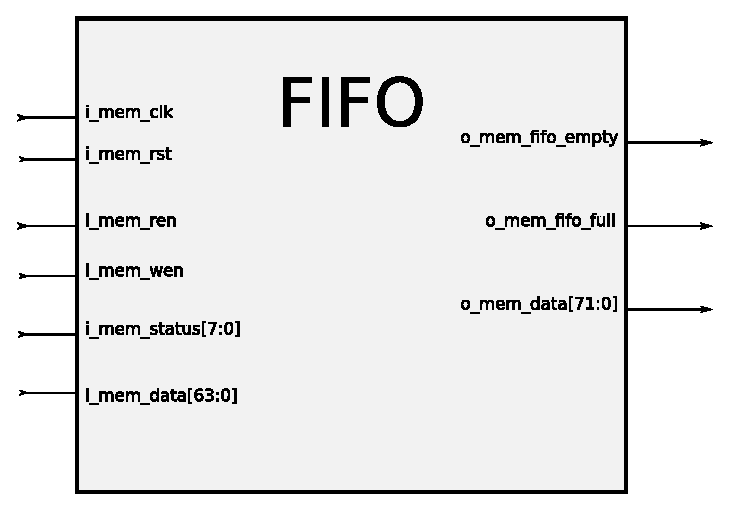
\includegraphics[scale=0.60]{figures/bloqfifo.eps}
\end{frame}

\begin{frame}{Delay Buffer}
\center 
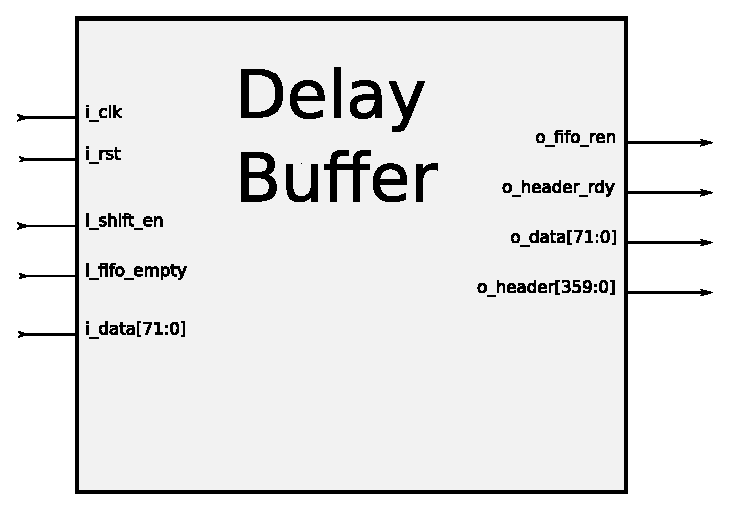
\includegraphics[scale=0.60]{figures/bloqdelaybuffer.eps}
\end{frame}

\begin{frame}{Uplink}
\center 
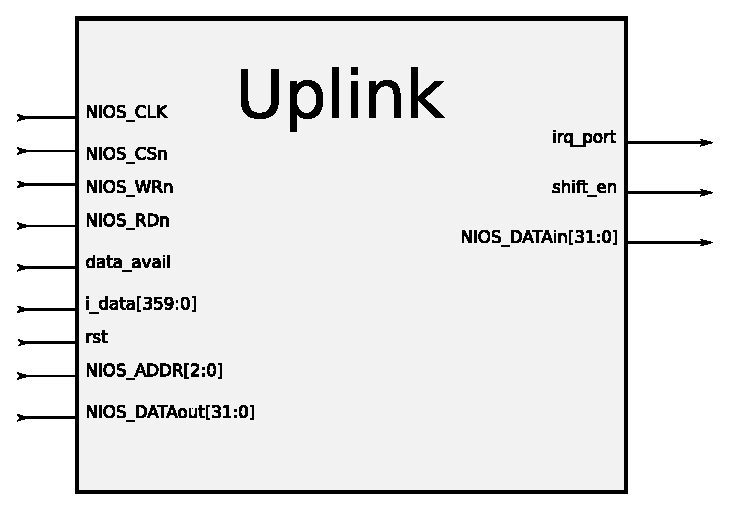
\includegraphics[scale=0.60]{figures/bloquplink.eps}
\end{frame}

\begin{frame}{Uplink}
  \begin{block}<+->{Uplink}
	\begin{itemize}
      \scriptsize
	\item La primera version de Uplink trasfiere al microprocesador toda la cabecera completa en 15 palabras de 32 bits. 
	\center
	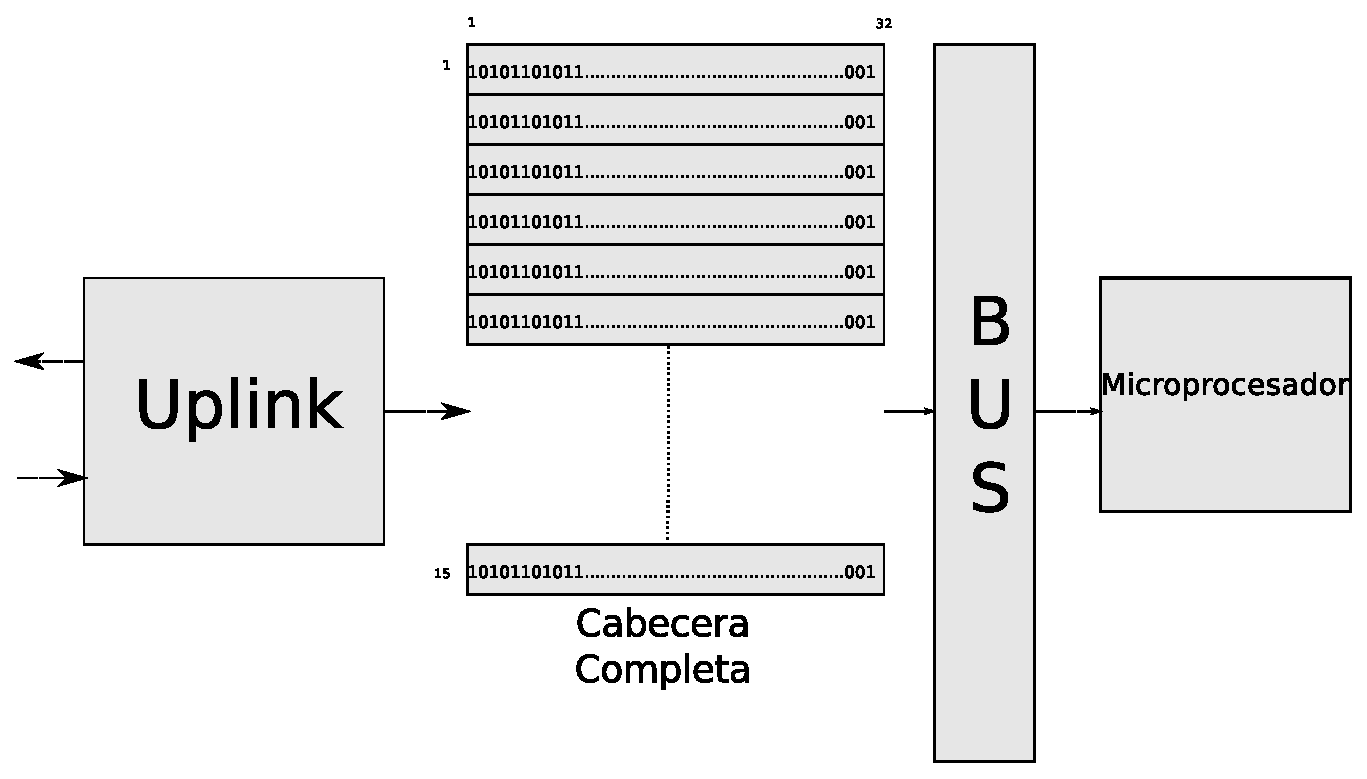
\includegraphics[scale=0.20]{figures/15pal.eps}  
	   \end{itemize}
	\begin{itemize}
      \scriptsize
	\item La segunda version de Uplink trasfiere al microprocesador solo la direccion IP destino en una palabra de 32 bits.
	\center
	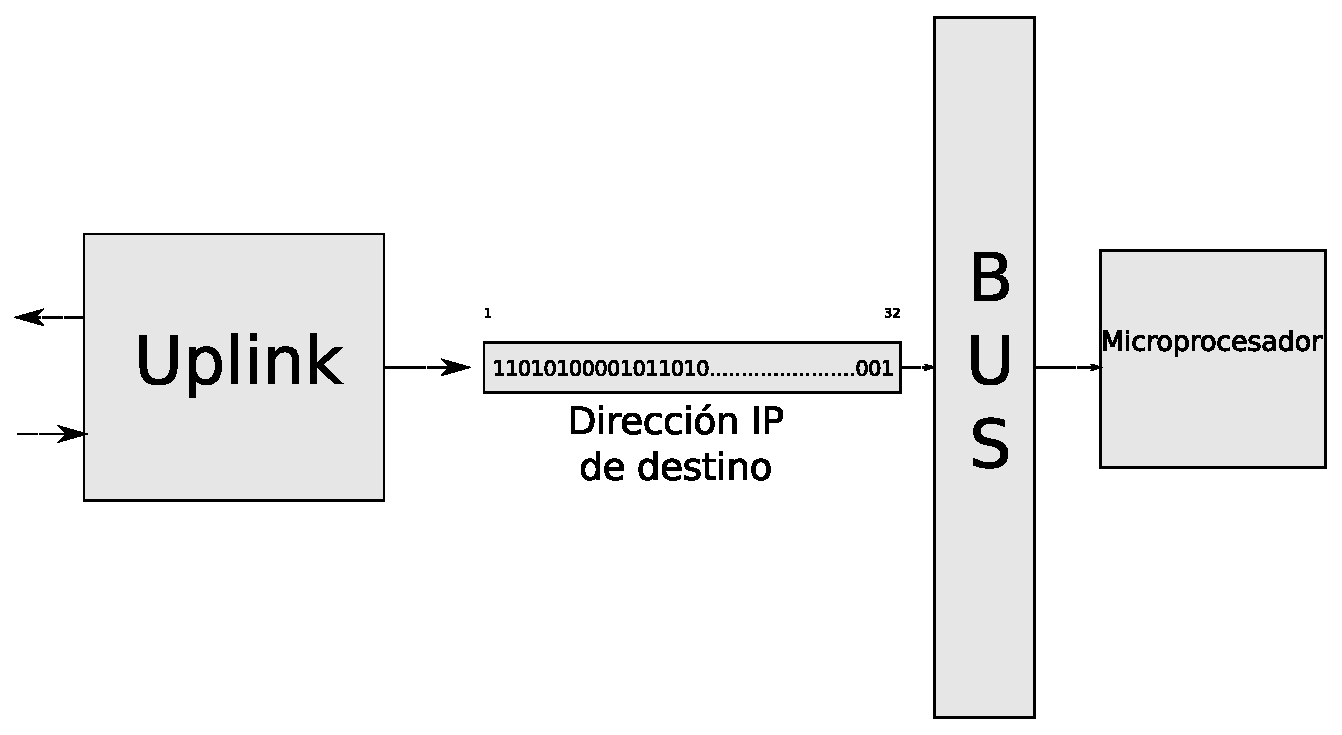
\includegraphics[scale=0.20]{figures/1pal.eps}
   \end{itemize}
\end{block}
\end{frame}


\begin{frame}{Write Output}
\center 
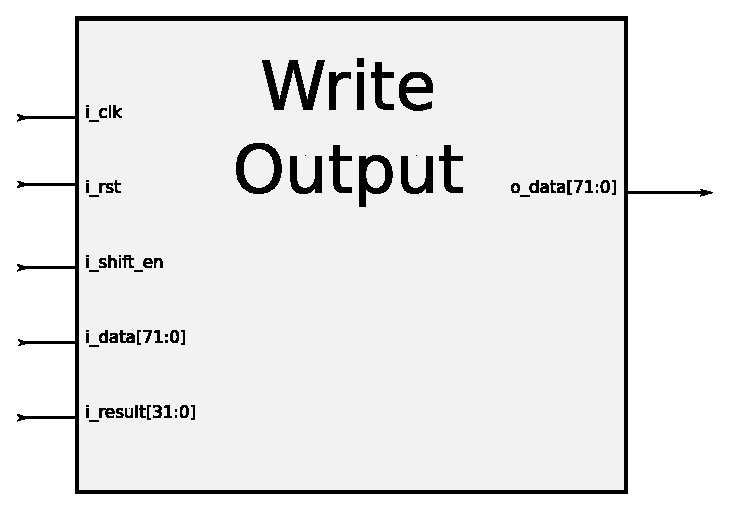
\includegraphics[scale=0.60]{figures/bloqwrite.eps}
\end{frame}

\section{Implementación}
\subsection{NIOS II}
\begin{frame}{Microprocesador NIOS II}
\center
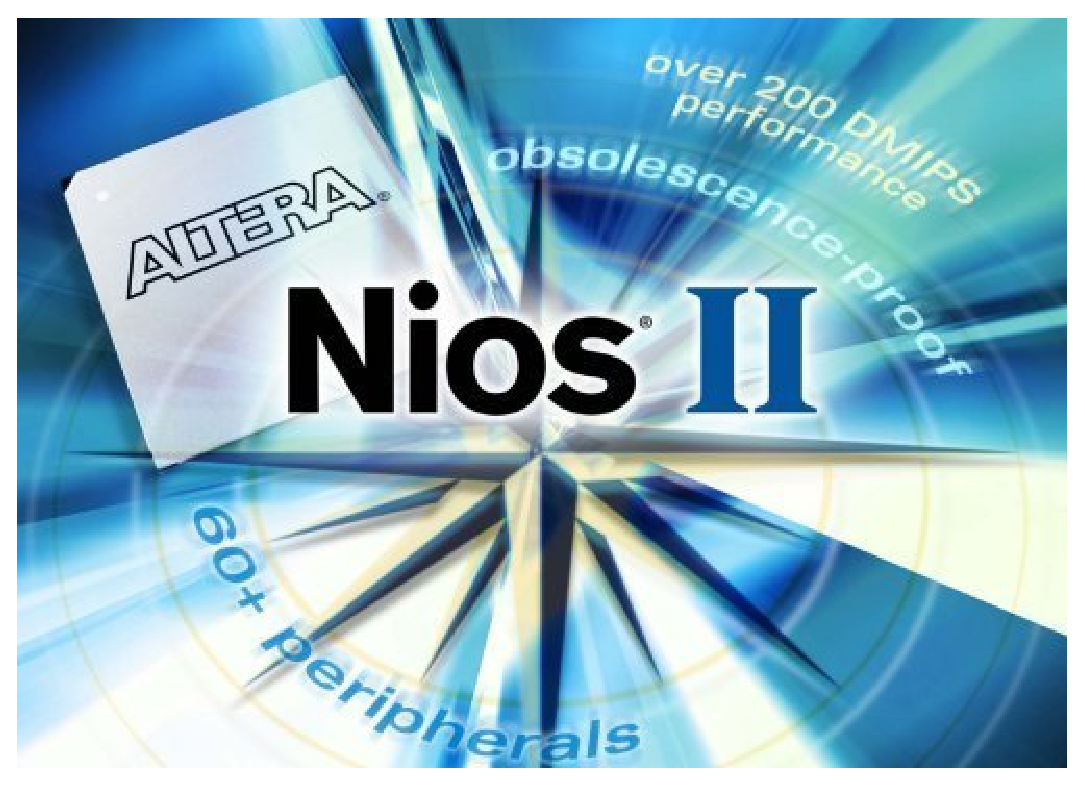
\includegraphics[scale=0.20]{figures/nios2.eps}
   \begin{block}<+->{NIOS II}	
    \begin{itemize}
	\scriptsize
     	\item Procesador RISC de 32 bits de proposito genera diseñado especificamente para la familia de FPGAs de Altera.
	\item Set de instrucciones, bus de datos y espacio de direcciones de 32 bits.
	\item Soporte de hasta 32 interrupciones.
	\item Entorno de desarrollo de software basado en GNU C/C++ integrado a Eclipse.
	\item Integración con SignalTap® II, el analizador de lógica embebida de Altera permitiendo el análisis  de todas las señales presentes en la FPGA.
	\item Set de instrucciones compatible entre todos las versiones del procesador Nios II.
	\item Multiplicación y división en una sola instrucción de 32 x 32 produciendo un resultado de 32-bits.
    \end{itemize}
	
  \end{block}
\end{frame}

\begin{frame}{Microprocesador NIOS II(cont)}
\center
   \begin{block}<+->{NIOS II}
	Es posible instanciar el procesador NIOS II en 3 diferentes configuraciones:	
	

    \begin{itemize}
	\scriptsize
     	\item Nios II/f, es un core optimizado para alcanzar el maximo rendimiento a expensas del tamaño del mismo.
	\item Nios II/s, esta diseñado para mantener el balance entre el rendimiento y el espacio ocupado dentro de la FPGA.
	\item Nios II/e, es un nucleo que busca utilizar la menor cantidad de logica para poder ser implementado en FPGAs de bajo costo.
    \end{itemize}
  \end{block}
\end{frame}

\subsection{Hardware}
\begin{frame}{Hardware}
  \begin{block}<+->{Placa de desarrollo DE2} 	
    \begin{itemize}
      \scriptsize
     	\item FPGA: Cyclone II EP2C35F672C6
	\item USB Blaster integrado, para configuración de FPGA
	\item Memoria: 8 MB SDRAM, 512 KB SRAM, 4 MB Flash
	\item Clock de 50 MHz
     \end{itemize}
  \end{block}

  \begin{block}<+->{FPGA Cyclone II EP2C35F672C6} 	
    \begin{itemize}
      \scriptsize
     	\item Elementos lógicos: 33216
	\item Bit totales de RAM: 483840
	\item Multiplicadores embebidos: 35
	\item PLLs: 4
	\item Cantidad máxima de pines definidos por el usuario: 475
     \end{itemize}
  \end{block}
\end{frame}

\subsection{Algoritmos}
\begin{frame}{Algoritmos}
\begin{block}<+->{LLU}   
    \begin{itemize}
      \scriptsize
     	\item Lenguaje: C++
     	\item Template \emph{list}
     	\item Cada nodo tiene 3 campos: Dirección de red, Máscara de red e Identificador de decisión
	\item Lista ordenada en base a longitud de máscara de red. Se recorre con un iterador
	\item En cada iteración, Realiza un AND con el valor de máscara del nodo que está siendo apuntado
	\item Si el resultado de la operación es igual al valor de dirección de red de dicho nodo, entonces se retorna con el valor identificador de decisión
	\item En otro caso, continúa la busqueda en el siguiente nodo
    \end{itemize}
  \end{block}
\end{frame}

\begin{frame}{Algoritmos}
\begin{block}<+->{UTL}   
    \begin{itemize}
      \scriptsize
     	\item Lenguaje: C++
     	\item Se implementaron clases propias, donde se definieron las características de los nodos del arbol, como así también las operaciones de inserción y búsqueda
     	\item Nodo \emph{común} y nodo \emph{decisión}
	\item Cada nodo tiene 2 campos: \emph{gw} y \emph{zero / one}
	\item El algoritmo de búsqueda toma como entrada la dirección IP de destino del paquete a clasificar
	\item Testeo bit a bit de la misma, partiendo con un puntero de recorrido desde el nodo raíz
	\item Si el bit de la dirección es 0 y el puntero \emph{zero} está apuntando hacia algún nodo, el puntero de recorrido se mueve al nodo apuntado por el puntero zero
	\item En caso contrario, se mueve al nodo apuntado por el puntero emph{one} (En caso de que exista alguno).
	\item El puntero de recorrido puede quedar en un nodo común o en un nodo decisión
	\item En cada iteración se debe guardar el valor de gw en caso de tratarse de un nodo decisión
    \end{itemize}
  \end{block}
\end{frame}

\subsection{Herramientas}
\begin{frame}{Herramientas de Desarrollo}
\begin{block}<+->{Quartus} 
	
    \begin{itemize}
      \scriptsize
     	\item IDE de Altera
	\item Incluye editor de textos y herramientas para síntesis
	\item Lenguaje HDL utilizado: Verilog HDL
    \end{itemize} 
	\center
	
\includegraphics[scale=0.10]{figures/Quartus.eps}  
  \end{block}
  \begin{block}<+->{Eclipse IDE for NIOS}   
	
    \begin{itemize}
      \scriptsize
     	\item Version de la IDE Eclipse adaptada para trabajar con el microprocesador NIOS II
	\item Lenguajes utilizados: C,C++
    \end{itemize}
	\center	
	
\includegraphics[scale=0.10]{figures/eclipse.eps}  	
  \end{block}
\end{frame}

\subsection{Verificación}

\begin{frame}{Uso de la FPGA}

	\center	
	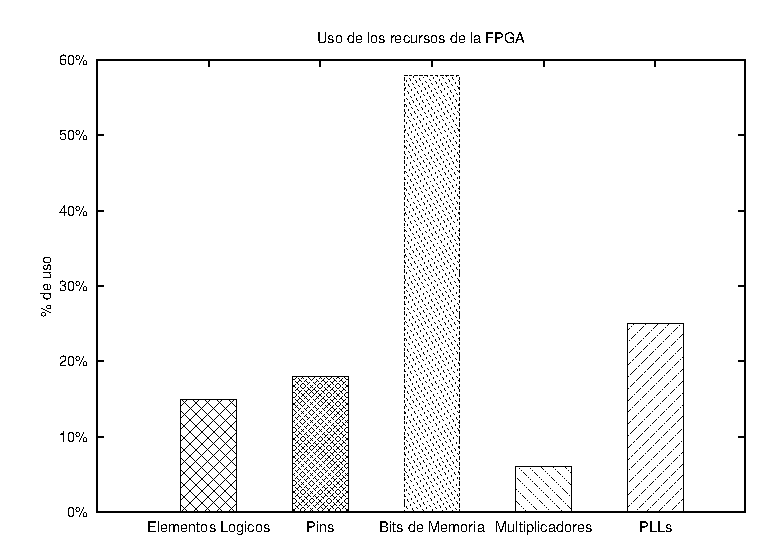
\includegraphics[scale=0.70]{figures/fpga.eps}  

\end{frame}


\begin{frame}{Verificación}
\begin{block}<+->{Etapas}   
    \begin{itemize}
      \scriptsize
     	\item 1º Paso: Módulo más simple (simpleRW)
     	\item 2º Paso: Implementación del modulo extractor. Debugging de señales.
     	\item 3º Paso: Integración extractor-software. LLU y UTL.
    \end{itemize}
  \end{block}
\end{frame}



\section{Resultados}
\subsection{Introducción}
\begin{frame}{Introducción}
	  \begin{block}<+->{Resultados}  
	\center 
	Se presentan los datos obtenidos de la ejecución del proyecto bajo ciertas condiciones representativas. Primero se estudiara el tiempo de 	respuesta de los algoritmos de manera individual, más tarde el rendimiento en la configuración mas simple, luego el sistema completo bajo condiciones 	varias y por ultimo el estudio de la mejora introducida por el uso de la cache. Para la obtencion de los datos que corresponden al sistema completo se utilizo el Script Python/Bash.
  \end{block}

\end{frame}

\subsection{Caso algoritmos unicamente}
\begin{frame}{Caso algoritmos unicamente} 
\center	
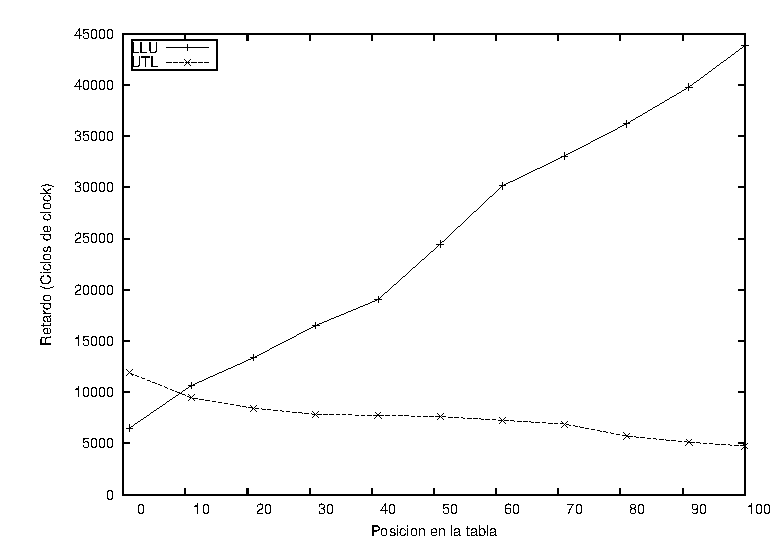
\includegraphics[scale=0.70]{figures/llu-utlsof.eps} 
\end{frame}

\subsection{Caso loopback}
\begin{frame}{Caso loopback} 
\center	
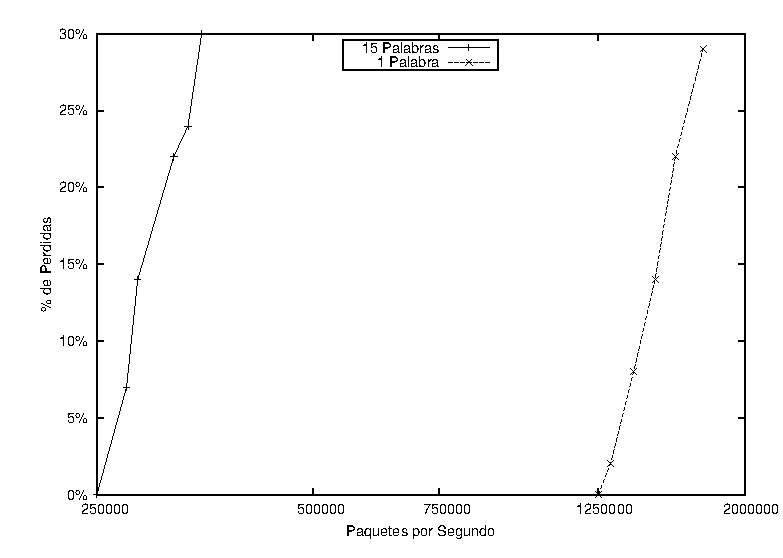
\includegraphics[scale=0.70]{figures/loop.eps} 
\end{frame}

\subsection{Implementacion completa}
\begin{frame}{Implementación completa: LLU} 
\center	
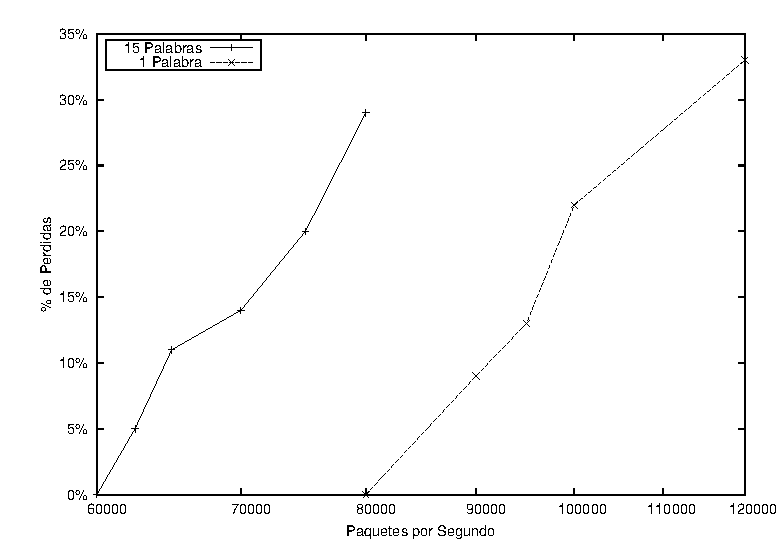
\includegraphics[scale=0.70]{figures/llumin.eps} 
\end{frame}


\begin{frame}{Implementación completa: LLU} 
\center	
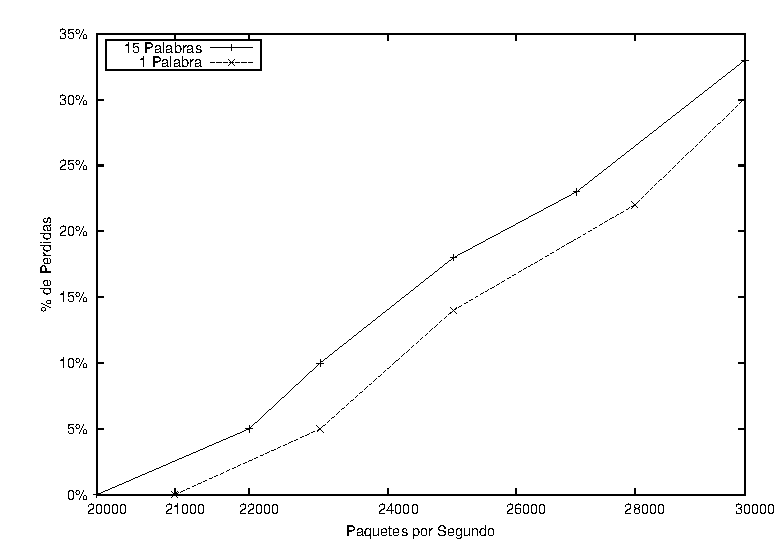
\includegraphics[scale=0.70]{figures/lluprom.eps} 
\end{frame}


\begin{frame}{Implementación completa: LLU} 
\center	
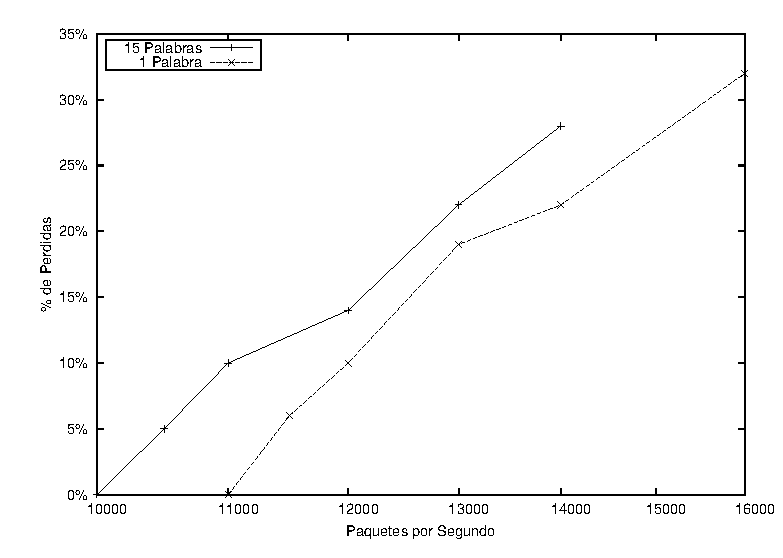
\includegraphics[scale=0.70]{figures/llumax.eps} 
\end{frame}


\begin{frame}{Implementación completa: UTL} 
\center	
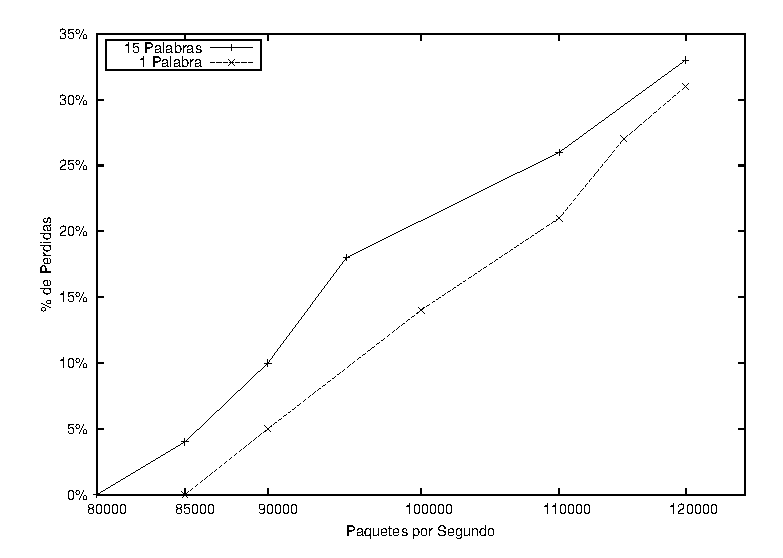
\includegraphics[scale=0.70]{figures/utlmin.eps} 
\end{frame}


\begin{frame}{Implementación completa: UTL} 
\center	
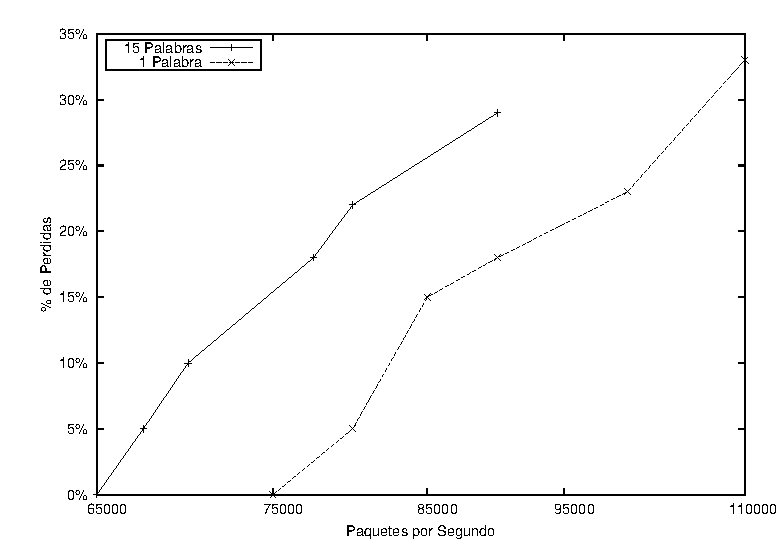
\includegraphics[scale=0.70]{figures/utlprom.eps} 
\end{frame}


\begin{frame}{Implementación completa: UTL} 
\center	
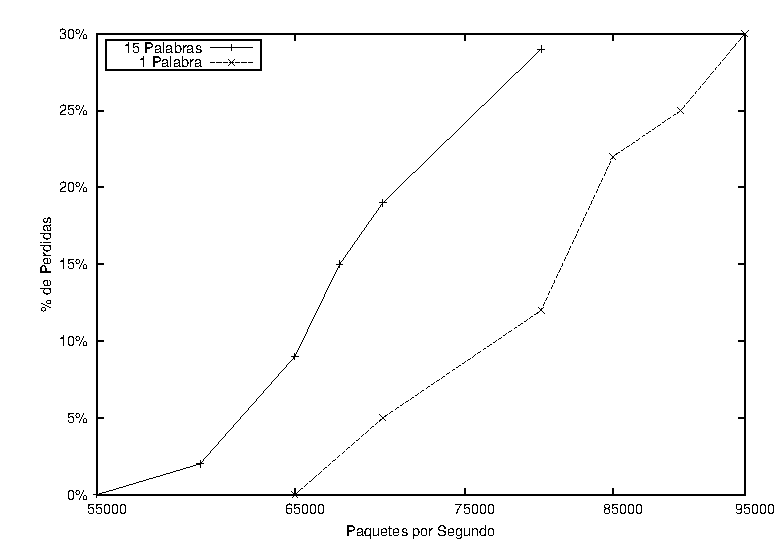
\includegraphics[scale=0.70]{figures/utlmax.eps} 
\end{frame}

\subsection{Comparativa inter-algortimos}
\begin{frame}{Comparativa inter-algortimos} 
\center	
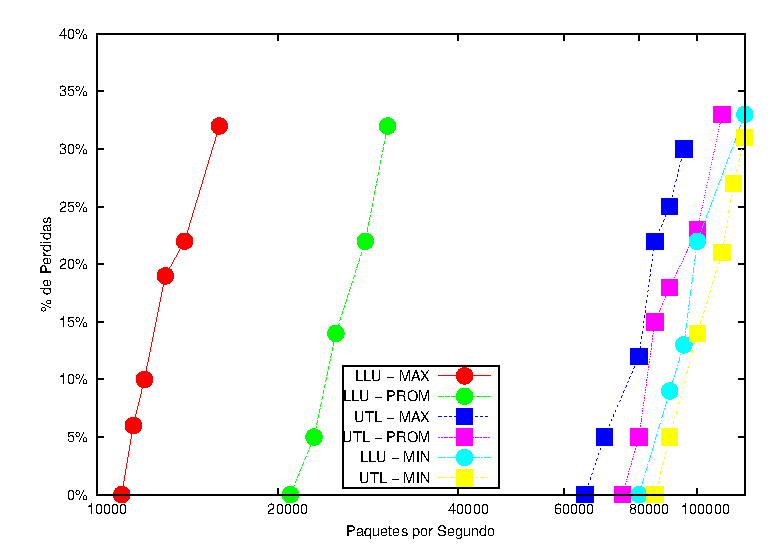
\includegraphics[scale=0.70]{figures/lluvsutl.eps} 
\end{frame}

\section{Conclusiones}
\begin{frame}{Conclusiones} 
\begin{block}<+->{Conclusiones}   
    \begin{itemize}
      \scriptsize
     	\item     	
    \end{itemize}
  \end{block}
\end{frame}

\end{document}
